\documentclass[11pt]{myclass}
\begin{document}
\subsection{Matlab Code for ODE-45 function call}
This the code chunk which integrates the 6DOF system of equations
\lstinputlisting[style=Matlab-editor]{ode_main.m}
\subsection{Matlab code for Drag}
Code chunk used to calculate the drag, this function is used in the body of the ode45 function and is used at every time step
\lstinputlisting[style=Matlab-editor]{drag1.m}
\subsection{Matlab code for Torque}
Code chunk to calculate the total torque acting on the coin,like drag,this function is also used in every time step of the ode45 routine
\lstinputlisting[style=Matlab-editor]{torque1.m}
\subsection{Matlab code for collision detection}
Event function to let MATLAB know when to stop integrating
\lstinputlisting[style=Matlab-editor]{collision.m}
Image showing the instance at which the solver stops and the position of the coin at that instance
\begin{figure}[H]
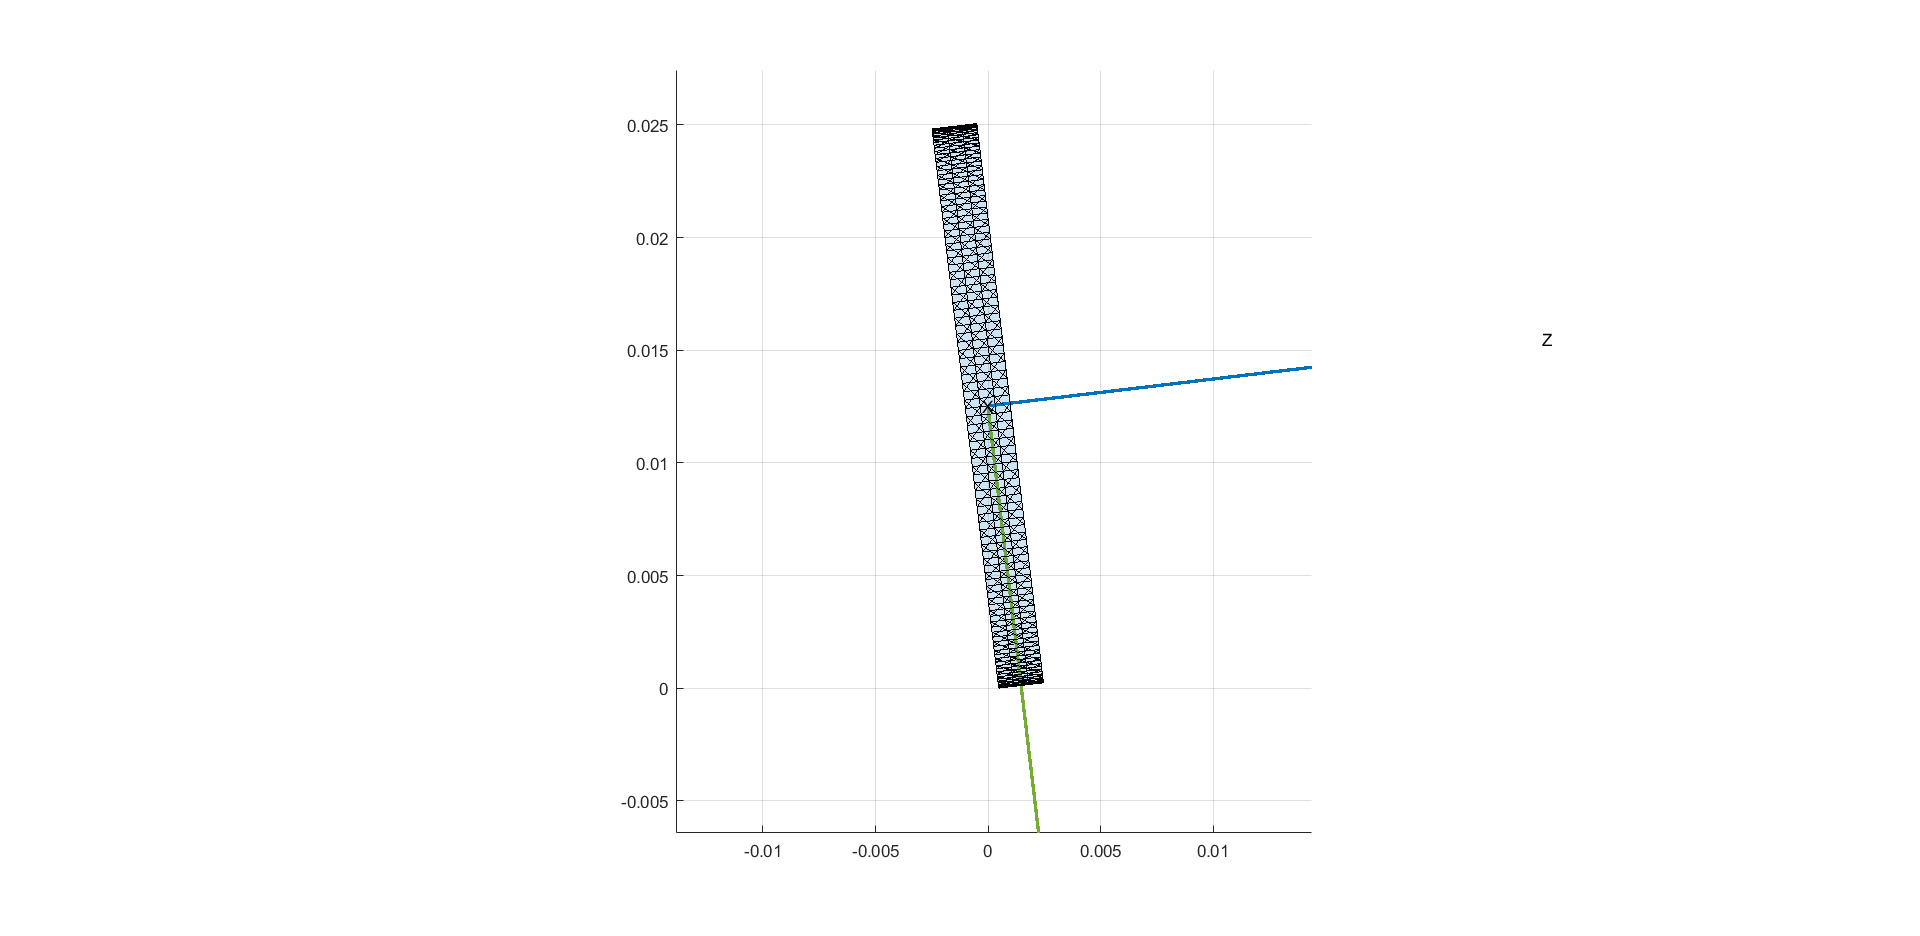
\includegraphics[scale = 0.25]{collision_photo.png}
\end{figure}
\subsection{Matlab code for finding out point of impact on coin}
Code chunk to solve for the position of the point which hits the floor, this information in needed for solving the impact equations
\lstinputlisting[style=Matlab-editor]{impact_point.m}
\subsection{Matlab code for solving impact equations}
Code chunk which solves the pre-impact-post-impact equations, I am sure I am making a major mistake here.( But i have not been able to figure what it is).
\lstinputlisting[style=Matlab-editor]{impact_solver.m}
\section{\textbf{Plots of free-fall and bouncing back}}
My plot for the freefall trajectory of the coin COM for two cases below
\begin{figure}[H]
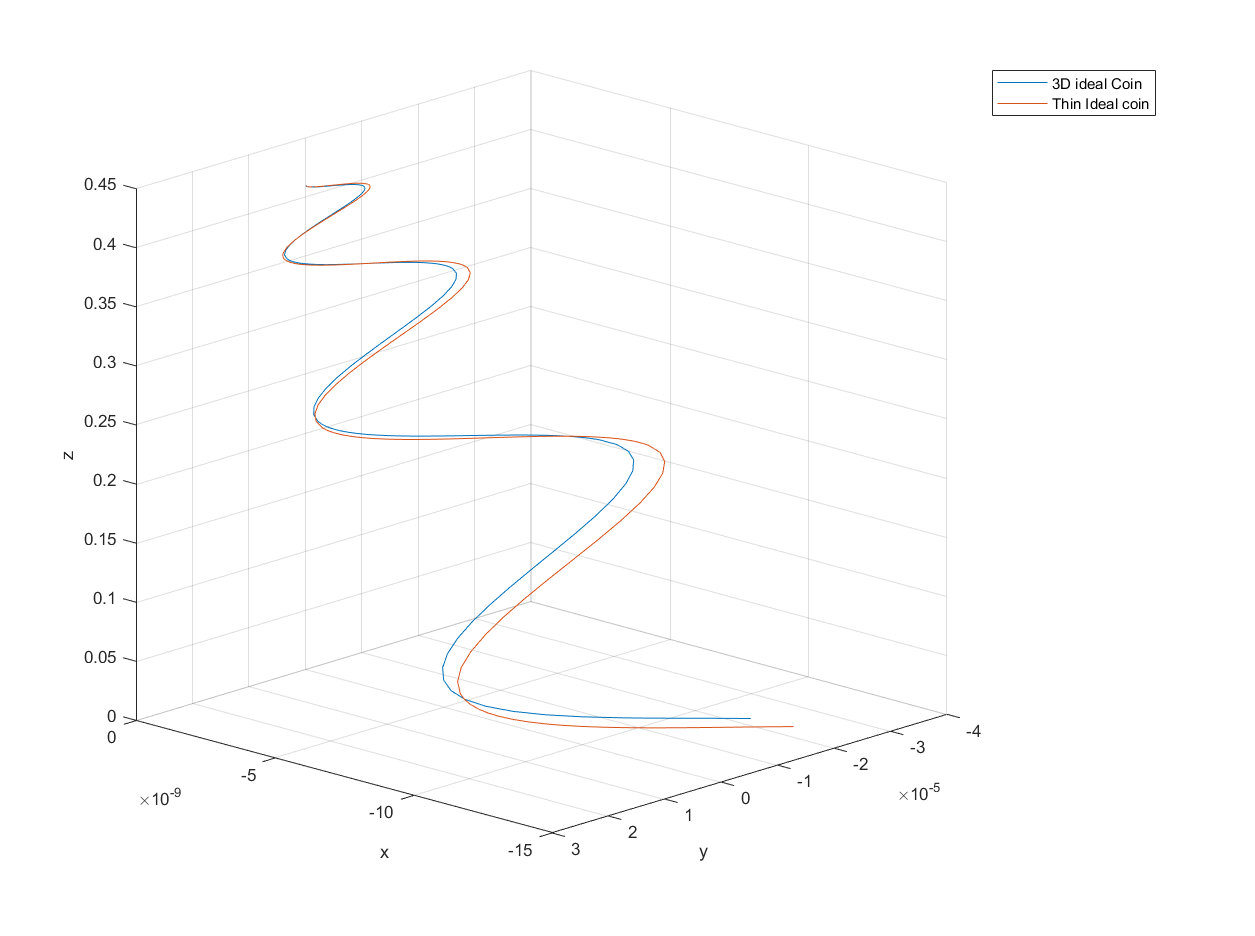
\includegraphics[scale = 0.4]{free_fall.png}
\end{figure}
Plots in paper for the same two cases below
\begin{figure}[H]
\includegraphics[scale = 0.85]{papers_free_fall_trajectory.png}
\end{figure}
Note:(The shapes of the plots match almost perfectly but there seems to be a mislabelling of the axes in the paper)\\

\section{Visualization of the coin motion}
\begin{figure}[H]
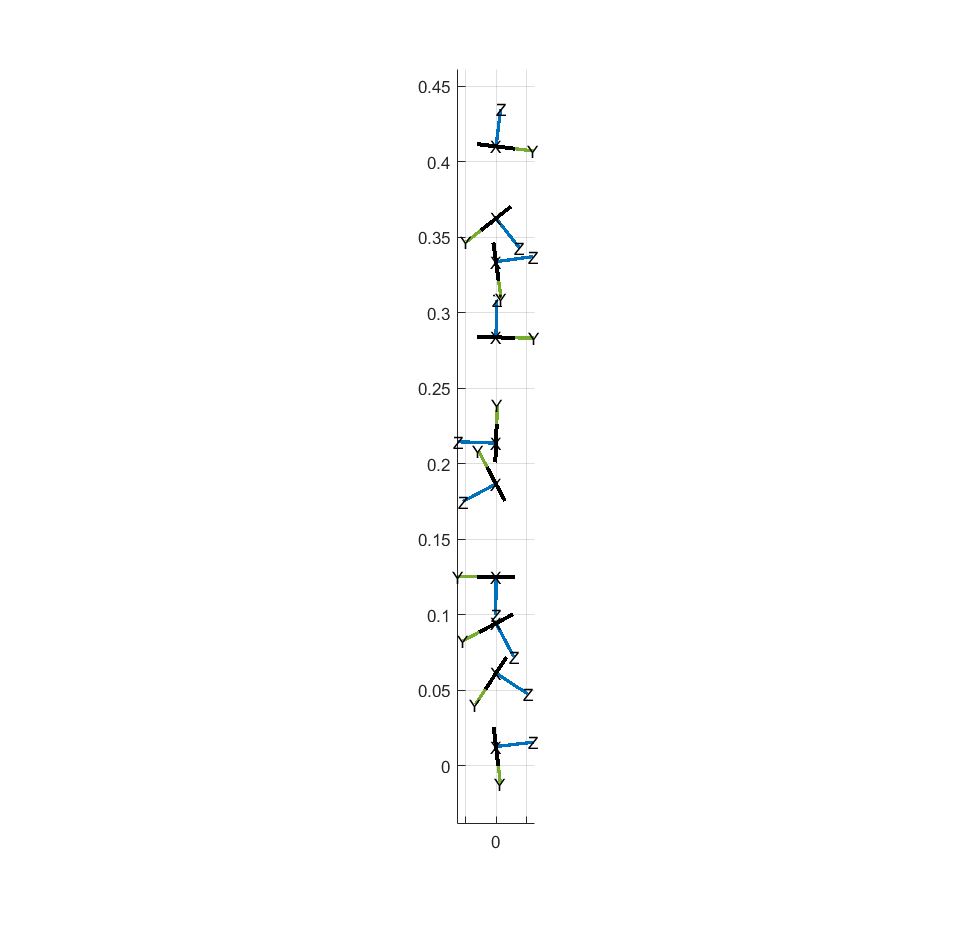
\includegraphics[scale = 0.85]{free_fall_projection.png}
\end{figure}
\begin{figure}[H]
\includegraphics[scale = 0.5]{free_fall_isometric.png}
\end{figure}
\subsection{\textbf{Plots of Bouncing Back}}
Note: (I attempted to simulate the impact,but i could only get coherent results for a single bounce, any more bounces were throwing a lot of errors and I have not been able to resolve them.)
Below is the image of one sucessful bounce i did get, It does not match the one in the paper however.
\begin{figure}[H]
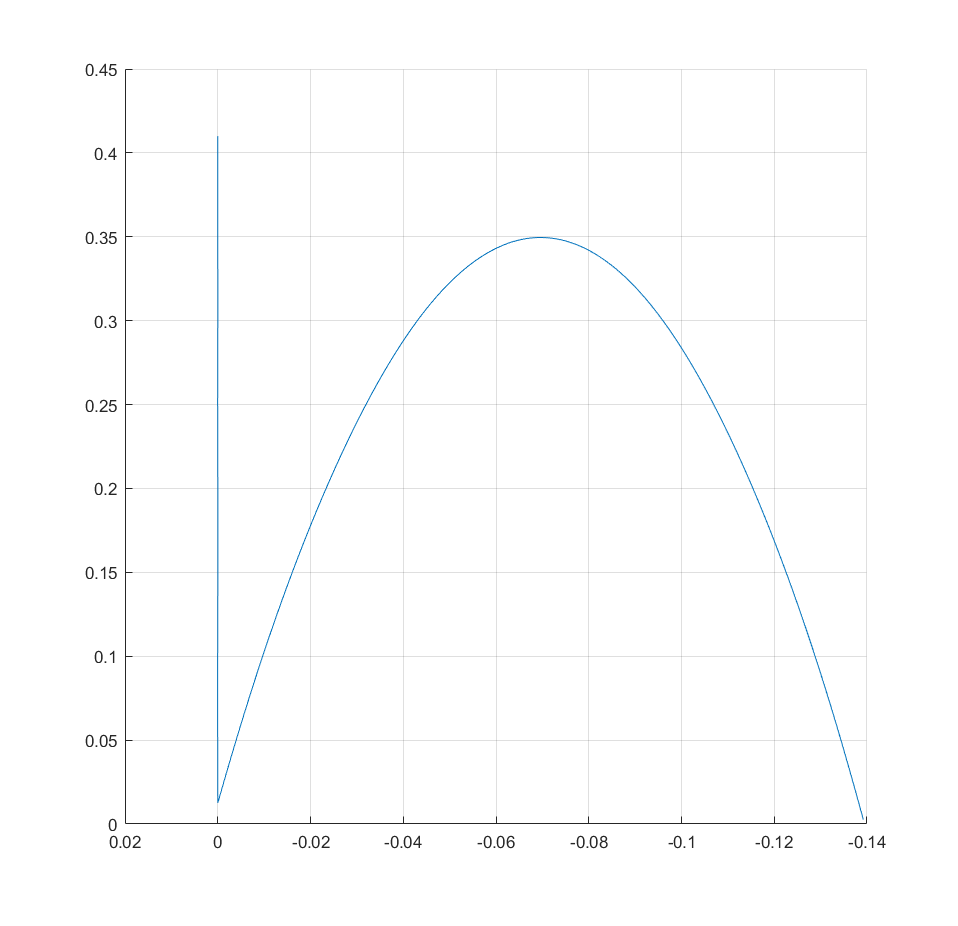
\includegraphics[scale = 0.5]{Bouncing_back.png}
\end{figure}
\end{document}